\chapter{Struttra del Magic Mirror}

Il Magic Mirror \`e un progetto ideato e sviluppato da Michael Teeuw, successivamente esteso nelle sue funzionalit\`a da una moltitudine di utenti su GitHub.
Una prima versione \`e stata scritta completamente in Python, mentre, in seguito, \`e stata creata una seconda versione nella quale si \`e preferito l'utilizzo di Electron,
che ha comportato una variazione di linguaggio, a favore di Javascript. In questo modo \`e stato possibile implementare un'interfaccia esteticamente pi\`u gradevole
e API pi\`u intuitive.
\\[2\baselineskip]

\section{Perch\`e Magic Mirror?}
L'idea dell'autore \`e nata rifacendosi allo specchio magico dell'omonima fiaba
scritta dai fratelli Grimm, La Bella Addormentata.\\
Il software viene mostrato attraverso un
comune monitor, trasmettendo immagini poste su uno sfondo completamente nero. Applicando sopra
una semplice pellicola a specchio (la quale da un lato permette di specchiarsi e dall'altro di vedere
attraverso) si crea un effetto particolare per cui una persona riesce a specchiarsi
e allo stesso tempo riesce a vedere le scritte o le immagini trasmesse dal monitor.
\\[2\baselineskip]
\begin{figure}[H]
    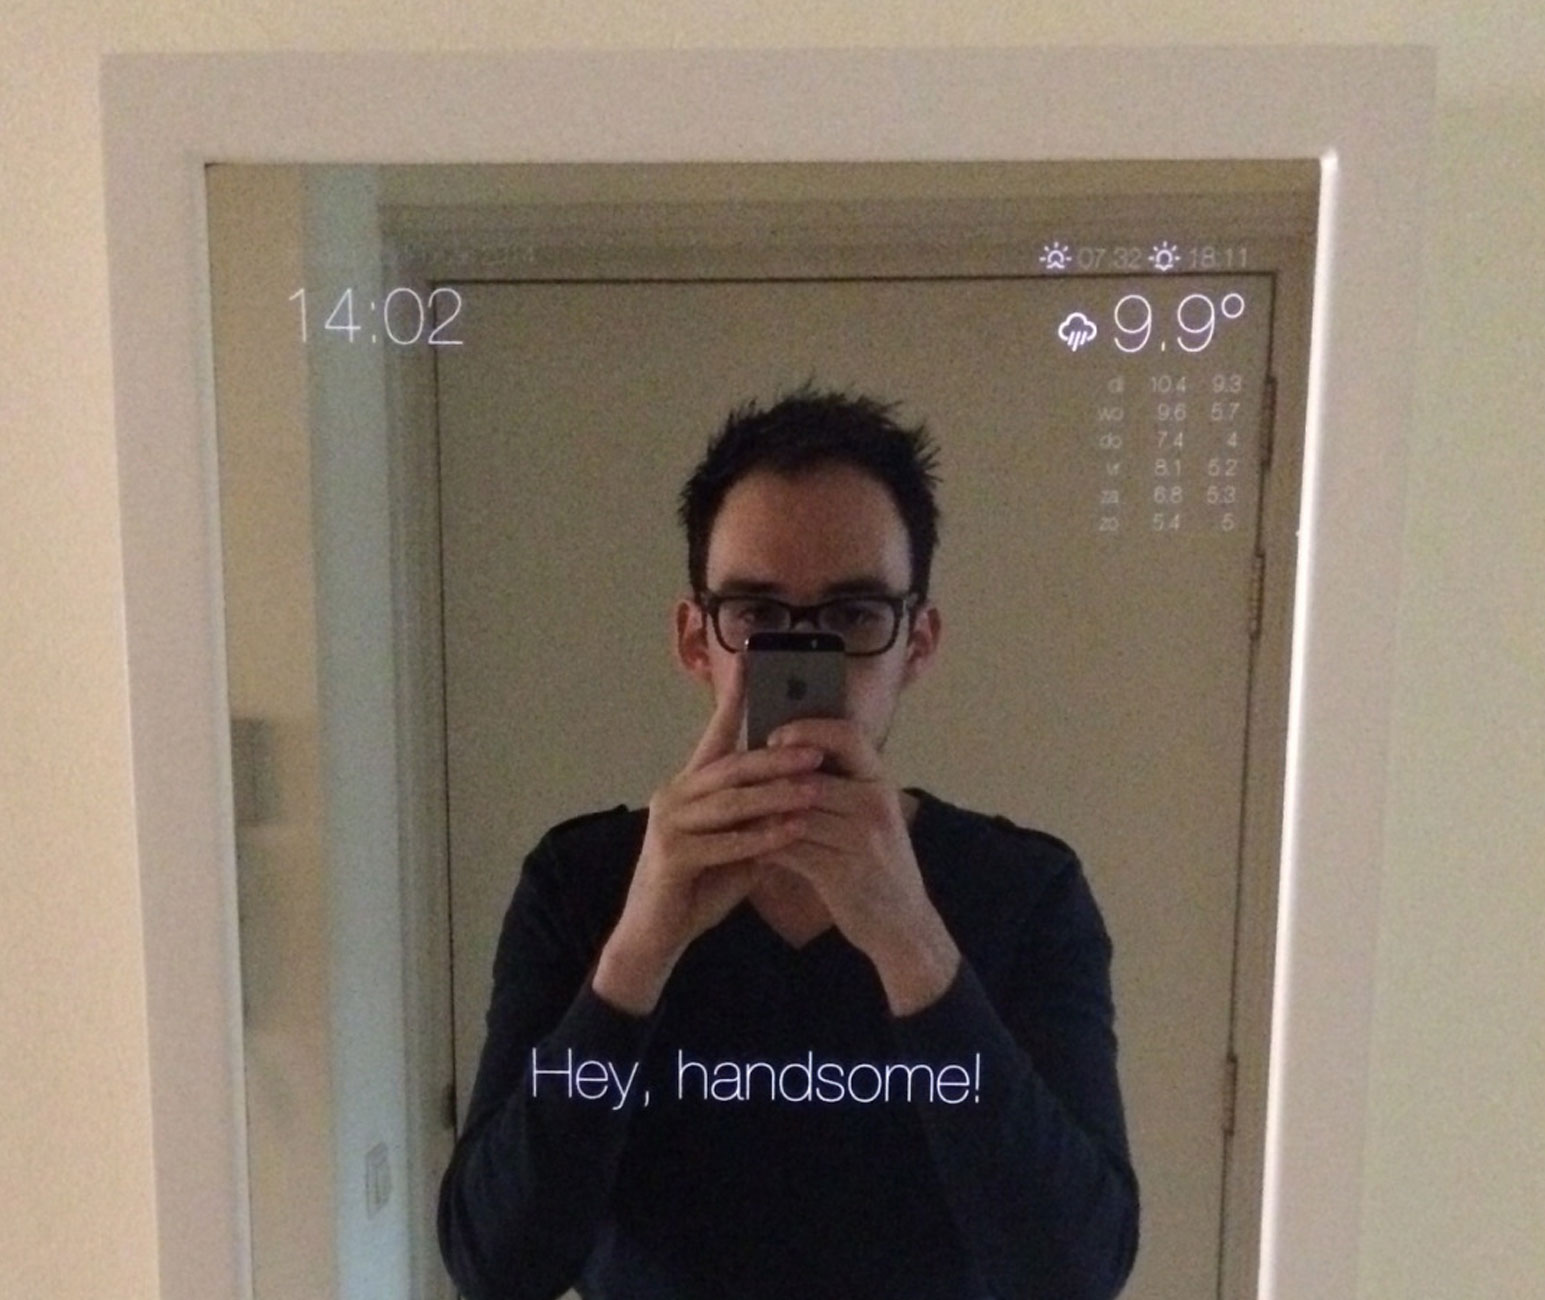
\includegraphics[width=1\textwidth, height=0.6\textheight]{magic_mirror}
    \caption{Magic Mirror by Michael Teeuw}
\end{figure}

\section{Avvio ed Escuzione}
Il Magic Mirror viene avviato tramite riga di comando di una shell: npm start, che va a ad eseguire
il codice di un file javascript indicato dal file package.json.
Il primo contiene il codice di Electron, che si occupa della creazione di una nuova finestra, che rappresenta l'interfaccia contenente il browser
contetente i Document Object Model(DOM), e il codice dell'applicazione, ovvero il corpo principale dello specchio.
Quest'ultima carica tutte le strutture dello specchio:
\begin{itemize}
\item le api per le applicazioni, che sono le interfacce usate per leggere e caricare le applicazioni inserite nel Magic Mirror.
\item le api per i Node Helper, interfacce per i Node Helper di una applicazione, sono strutture opzionali usate per collegamenti
esterni al Magic Mirror(per esempio con api di un servizio cloud). Ogni applicazione ha il proprio Node Helper con cui pu\`o comunicare tramite messaggi in modo
simile a come comunicano le applicazioni tra di loro.
\item un "Socket", entit\`a principale che definisce le funzioni e le metodologie per lo scambio dei messaggi tra le applicazioni e i rispettivi Node Helper.
\item un Logger, implementato per tenere i log dell'applicazione e degli evenutali errori. Usato pricipalemnte per il debugging.
\item un file Config, un file di configurazione dello specchio, nel quale sono segnate il nome e le coordinate per la posizione all'inteno della pagina\\[2\baselineskip]
\end{itemize}
Inoltre viene inzializzato un server il quale ha il compito di trasmettere la pagina renderizzata sulla base
degli output delle varie applicazioni al browser avviato inizialmente.

\subsection{Il file di Configurazione}
Come gi\`a menzionato il Magic Mirror carica un file di configurazione, il quale ha al suo inteno:
\begin{itemize}
\item la porta del server
\item una whitelist ovvero un ip oppure un range di ip che possono collegarsi allo specchio
\item la lingua principale del sistema
\item il formato del timer (12h o 24h)
\item unit\`a di misura usata (per esmepio metrica)
\item una lista di applicazioni (in formato JSON) da caricare con la relativa posizione nella pagina. Necessarimaente per ogni applicazione deve comparire il
nome e la posizione, opzionalmente si possono inserire un campo header e un campo config specifico per l'applicazione:
\begin{lstlisting}
{
	"module": 'nome dell'applicazione',
	"position": 'la posizione dell'applicazione all'intenro dello specchio',
	"header": 'stampa sopra all'applicazione',
	"config": { opzioni varie in formato JSON }
}
\end{lstlisting}
\end{itemize}
La lingua, il formato del timer e l'unit\`a di misura usata sono strumenti che possono essere utilizzati nella creazione di un'applicazione
(per esempio il display di un orologio).

\section{Specifiche delle applicazioni}
La modifica del file di configurazione, appena descritta, del Magic Mirror serve per notificare la presenza delle applicazioni a quest'ultimo,
ma perch\`e possano funzionare \`e necessario che si trovino in una specifica cartella e rispettino delle specifiche regole.
Per inserire il codice dell'applicazione all'interno dello specchio \`e necessario creare una cartella con uno nome identificativo dell'applicazione
nella directory "Modules".
Dentro la cartella appena creata devono essere inseriti:
\begin{itemize}
\item 1 file Javascript(JS), il documento principale con lo stesso nome della cartella appena creata, contiene il codice il codice dell'applicaizone, il quale
conterr\`a ance il codice per la creazione dei DOM
\item 1 file Cascading Style Sheets(CSS), opzionale, per modificare l'esetica del DOM della relativa applicazione
\item 1 file node\_helper.js, opzionale, che \`e il Node Helper associato alla specifica applicazione
\item Altri file necessari all'applicazione (immagini, json, ecc...)\\[1\baselineskip]
\end{itemize}
Il file javascript principale viene caricato per primo dal Magic Mirror, ed \`e composto dalla chiamata una funzione passando due parametri:
\begin{lstlisting}[language=JavaScript]
{
	Module.register("Nome del Modulo", { /* lista JSON di oggetti contenenti funzioni o variabili */});
}
\end{lstlisting}
Il primo parametro \`e una stringa che rappresenta il nome del modulo, il quale deve essere necessariamente uguale a quello della cartella e del file Javascript,
mentre il secondo \`e una lista JSON contenente funzioni o variabili (come in figura x).
Le funzioni offerte dalle API sono:
\begin{itemize}
\item defaults: {}, una lista di variabili che possono essere richiamate all'interno di una qualsiasi funzione tramite il comando "this.config.variabile".
I valori di queste possono essere sovrascritti modificando il campo "config" del relativo modulo nel file di configurazione del Magic Mirror.
\item start: function(){}, funzione che viene eseguita quando tutte le applicazioni dello specchio sono state caricate (ovvero sono stati creati tutti i relativi DOM)
\item getDom: function(){}, funzione che deve ritornare 1 DOM, un oggetto HTML contenente i dati da mostrare a schermo, creato tramite funzioni di Javascript
\item getStyles: function() { return []}, funzione che ritorna un array di file (in formato css) usati per l'estetica del DOM. Possono essere nella cartella dell'applicazione
oppure ottenuti tramite link
\item getTranslations: function() {	return {en: "translations/en.json", de: "translations/de.json"}}, funzione per tradurre l'applicazione in pi\`u lingue,
se disponibile viene caricata la traduzione in base alla lingua configurata nel software
\item getHeader: function() {	return this.data.header;}, funzione che stampa il campo "header" della configurazione, con la possibilit\`a concaternarla
ad una stringa o ad un parametro
\item notificationReceived: function(notification, payload, sender) {}, funzione che serve per ricevere messaggi ad altre applicazioni. Viene richiamata alla ricezione
\item socketNotificationReceived: function(notification, payload){}, funzione analoga alla precedente, ma il messaggio \`e ricevuto dal Node Helper della relativa applicazione\\[1\baselineskip]
\end{itemize}
Inoltre possono essere aggiunte delle funzioni necessarie all'applicazione implementandole con la stessa sintassi di quelle di default.
\\[1\baselineskip]
Il Node Helper, invece, viene caricato come libreria ed esportato insieme all'applicazione quando viene caricata dallo specchio, quindi per inizializzarlo bisogna
inserire:
\begin{lstlisting}[language=JavaScript]
{
  var NodeHelper = require("node_helper");
  module.exports = NodeHelper.create({/* lista JSON di oggetti contenenti funzioni*/});
}
\end{lstlisting}
A differenza del file Javascript principale, l'unica funzione messa a disposizione dall' API \`e:
\begin{lstlisting}[language=JavaScript]
{
  start: function() {}
}
\end{lstlisting}
mentre \`e possibile implementare le proprie funzioni con la stessa sintassi.

\section{Messaggistica del MM}
In precedenza \`e stato gi\`a accennato che il Magic Mirror implementa un meccanismo di messaggistica sfruttando un sistema di socket integrato,
utile per l'organizzazione e la moderazione delle applicazioni tramite l'utilizzo di funzioni messe a disposizione dell'API.
Le funzioni usate per ricevere i messaggi, come gi\`a accennato nella sezione precedente, sono: \textit{socketNotificationReceived(notification, payload)},
per la ricezione dei messagi da parte del Node Helper, e \textit{notificationReceived(notification, payload, sender)}, per la ricezione di
messaggi dalle altre applicazioni.
Per spedirli vengono chiamate le funzioni \textit{sendSocketNotification(notification, payload)} e \textit{sendNotificationReceived(notification, payload, sender)},
i cui campi dinicano:
\begin{itemize}
\item notification, l'indentificatore della notifica, una sorta di header al quale si pu\`o assegnare un qualunque oggetto
\item payload, il corpo del messaggio, \`e un campo opzionale
\item sender, usato solo nei messaggi tra i mouduli, riporta l'identificativo dell'applicazione che lo ha mandato\\[1\baselineskip]
\end{itemize}
\textit{sendNotificationReceived} a differenza del suo corrispettivo per il Node Helper, manda il messaggio in broadcast a tutte le applicazioni attive
sulla macchina, e deve essere filtrato dalle singole in base al campo \textit{notification}
